
\let\negmedspace\undefined
\let\negthickspace\undefined
\documentclass[journal,12pt,twocolumn]{IEEEtran}
\usepackage{cite}
\usepackage{amsmath,amssymb,amsfonts,amsthm}
\usepackage{algorithmic}
\usepackage{graphicx}
\usepackage{textcomp}
\usepackage{xcolor}
\usepackage{txfonts}
\usepackage{listings}
\usepackage{enumitem}
\usepackage{mathtools}
\usepackage{gensymb}
\usepackage[breaklinks=true]{hyperref}
\usepackage{tkz-euclide} % loads  TikZ and tkz-base
\usepackage{listings}



\newtheorem{theorem}{Theorem}[section]
\newtheorem{problem}{Problem}
\newtheorem{proposition}{Proposition}[section]
\newtheorem{lemma}{Lemma}[section]
\newtheorem{corollary}[theorem]{Corollary}
\newtheorem{example}{Example}[section]
\newtheorem{definition}[problem]{Definition}
%\newtheorem{thm}{Theorem}[section] 
%\newtheorem{defn}[thm]{Definition}
%\newtheorem{algorithm}{Algorithm}[section]
%\newtheorem{cor}{Corollary}
\newcommand{\BEQA}{\begin{eqnarray}}
\newcommand{\EEQA}{\end{eqnarray}}
\newcommand{\define}{\stackrel{\triangle}{=}}
\theoremstyle{remark}
\newtheorem{rem}{Remark}
%\bibliographystyle{ieeetr}
\begin{document}
%
\providecommand{\pr}[1]{\ensuremath{\Pr\left(#1\right)}}
\providecommand{\prt}[2]{\ensuremath{p_{#1}^{\left(#2\right)} }}        % own macro for this question
\providecommand{\qfunc}[1]{\ensuremath{Q\left(#1\right)}}
\providecommand{\sbrak}[1]{\ensuremath{{}\left[#1\right]}}
\providecommand{\lsbrak}[1]{\ensuremath{{}\left[#1\right.}}
\providecommand{\rsbrak}[1]{\ensuremath{{}\left.#1\right]}}
\providecommand{\brak}[1]{\ensuremath{\left(#1\right)}}
\providecommand{\lbrak}[1]{\ensuremath{\left(#1\right.}}
\providecommand{\rbrak}[1]{\ensuremath{\left.#1\right)}}
\providecommand{\cbrak}[1]{\ensuremath{\left\{#1\right\}}}
\providecommand{\lcbrak}[1]{\ensuremath{\left\{#1\right.}}
\providecommand{\rcbrak}[1]{\ensuremath{\left.#1\right\}}}
\newcommand{\sgn}{\mathop{\mathrm{sgn}}}
\providecommand{\abs}[1]{\left\vert#1\right\vert}
\providecommand{\res}[1]{\Res\displaylimits_{#1}} 
\providecommand{\norm}[1]{\left\lVert#1\right\rVert}
%\providecommand{\norm}[1]{\lVert#1\rVert}
\providecommand{\mtx}[1]{\mathbf{#1}}
\providecommand{\mean}[1]{E\left[ #1 \right]}
\providecommand{\cond}[2]{#1\middle|#2}
\providecommand{\fourier}{\overset{\mathcal{F}}{ \rightleftharpoons}}
\newenvironment{amatrix}[1]{%
  \left(\begin{array}{@{}*{#1}{c}|c@{}}
}{%
  \end{array}\right)
}
%\providecommand{\hilbert}{\overset{\mathcal{H}}{ \rightleftharpoons}}
%\providecommand{\system}{\overset{\mathcal{H}}{ \longleftrightarrow}}
	%\newcommand{\solution}[2]{\textbf{Solution:}{#1}}
\newcommand{\solution}{\noindent \textbf{Solution: }}
\newcommand{\cosec}{\,\text{cosec}\,}
\providecommand{\dec}[2]{\ensuremath{\overset{#1}{\underset{#2}{\gtrless}}}}
\newcommand{\myvec}[1]{\ensuremath{\begin{pmatrix}#1\end{pmatrix}}}
\newcommand{\mydet}[1]{\ensuremath{\begin{vmatrix}#1\end{vmatrix}}}
\newcommand{\myaugvec}[2]{\ensuremath{\begin{amatrix}{#1}#2\end{amatrix}}}
\providecommand{\rank}{\text{rank}}
\providecommand{\pr}[1]{\ensuremath{\Pr\left(#1\right)}}
\providecommand{\qfunc}[1]{\ensuremath{Q\left(#1\right)}}
	\newcommand*{\permcomb}[4][0mu]{{{}^{#3}\mkern#1#2_{#4}}}
\newcommand*{\perm}[1][-3mu]{\permcomb[#1]{P}}
\newcommand*{\comb}[1][-1mu]{\permcomb[#1]{C}}
\providecommand{\qfunc}[1]{\ensuremath{Q\left(#1\right)}}
\providecommand{\gauss}[2]{\mathcal{N}\ensuremath{\left(#1,#2\right)}}
\providecommand{\diff}[2]{\ensuremath{\frac{d{#1}}{d{#2}}}}
\providecommand{\myceil}[1]{\left \lceil #1 \right \rceil }
\newcommand\figref{Fig.~\ref}
\newcommand\tabref{Table~\ref}
\newcommand{\sinc}{\,\text{sinc}\,}
\newcommand{\rect}{\,\text{rect}\,}
%%
%	%\newcommand{\solution}[2]{\textbf{Solution:}{#1}}
%\newcommand{\solution}{\noindent \textbf{Solution: }}
%\newcommand{\cosec}{\,\text{cosec}\,}
%\numberwithin{equation}{section}
%\numberwithin{equation}{subsection}
%\numberwithin{problem}{section}
%\numberwithin{definition}{section}
%\makeatletter
%\@addtoreset{figure}{problem}
%\makeatother

%\let\StandardTheFigure\thefigure
\let\vec\mathbf
\begin{table}[h!]
 \begin{center}
  \caption{Table 1}
  \label{tab: table1}
\begin{tabular}{|l|c|r|}
    \hline
    Parameter & Values & Description\\
    \hline
     $\vec{m_1}$ & $\myvec{7\\-1\\}$ & $AB$\\
     $\vec{m_2}$ & $\myvec{-6\\2\\}$ & $BC$\\
     $\vec{m_3}$ & $\myvec{-1\\-1\\}$ & $CA$\\
    \hline
    $\norm{\vec{B}-\vec{A}}$ & $7.071$ & length of $AB$\\
    $\norm{\vec{C}-\vec{B}}$ & $6.324$ & length of $BC$\\
    $\norm{\vec{A}-\vec{C}}$ & $1.414$ & length of $CA$\\
    \hline
    rank & 3 & non collinear\\
    \hline
    $\vec{n_1}$ & $\myvec{-2\\-6\\}$ & $AB$\\
    ${c_1}$ & $-26$ & {}\\
    $\vec{n_2}$ & $\myvec{1\\-1\\}$ & $BC$\\
    ${c_2}$ & $-7$ & {}\\
    $\vec{n_3}$ & $\myvec{1\\7\\}$ & $CA$\\
    ${c_3}$ & $25$ & {}\\
    \hline
    Area & $4$ & Area of triangle\\
    \hline
    $\angle A$ & $53.13\degree$ & {}\\
    $\angle B$ & $10.30\degree$ & Angle\\
    $\angle C$ & $116.56\degree$ & {}\\
    \hline
\end{tabular}
\end{center}
\end{table}
\begin{figure}[h!]
\centering

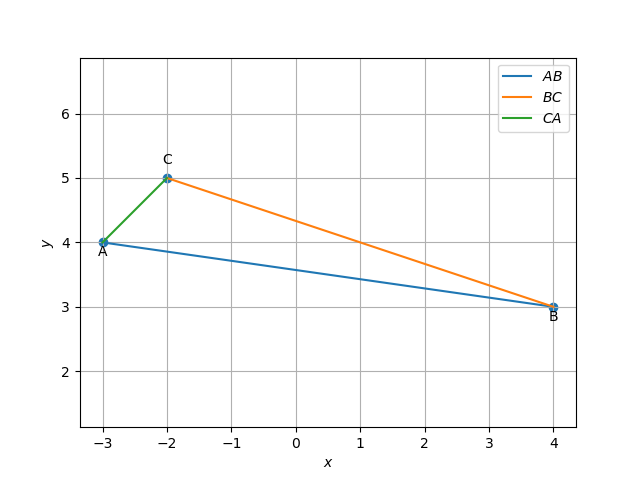
\includegraphics[width=\columnwidth] {./figs/fig17.png}
\caption{Figure 1}
\label{fig1: sides}
\end{figure}
\begin{table}[h!]
 \begin{center}
  \caption{Table 2}
  \label{tab: table2}
\begin{tabular}{|l|c|r|}
    \hline
    Parameter & Values & Description\\
    \hline
    $\vec D$ & $\myvec{1\\4\\}$ & {}\\
    $\vec E$ & $\myvec{\frac{-5}{2}\\\frac{9}{2}\\}$ & Mid-points\\
    $\vec F$ & $\myvec{\frac{1}{2}\\\frac{7}{2}\\}$ & {}\\
    \hline
    $\vec {n_1}$ & $\myvec{0\\-4\\}$ & $AD$\\
    ${c_1}$ & -16 & {}\\
    $\vec {n_2}$ & $\myvec{\frac{3}{2}\\\frac{13}{2}\\}$ & $BE$\\
    ${c_2}$ & $\frac{51}{2}$ & {}\\
    $\vec {n_3}$ & $\myvec{\frac{-3}{2}\\\frac{-5}{2}\\}$ & $CF$\\
    ${c_3}$ & $\frac{-19}{2}$ & {}\\
    \hline
    $\vec G$ & $\myvec{\frac{-1}{3}\\4\\}$ & Centroid\\
    \hline
    $\frac{GA}{DG}$ & 2 & {}\\
    $\frac{GB}{EG}$ & 2 & Equal\\
    $\frac{GC}{FG}$ & 2 & {}\\
    \hline
    rank & 2 & collinear\\
    \hline
    $\norm{\vec{A}-\vec{F}}$ & $\myvec{\frac{-7}{2}\\\frac{1}{2}\\}$ & Equal\\
    $\norm{\vec{E}-\vec{D}}$ & $\myvec{\frac{-7}{2}\\\frac{1}{2}\\}$ & Hence a parallelogram\\
    \hline
\end{tabular}
\end{center}
\end{table}
\begin{figure}[h!]
\centering

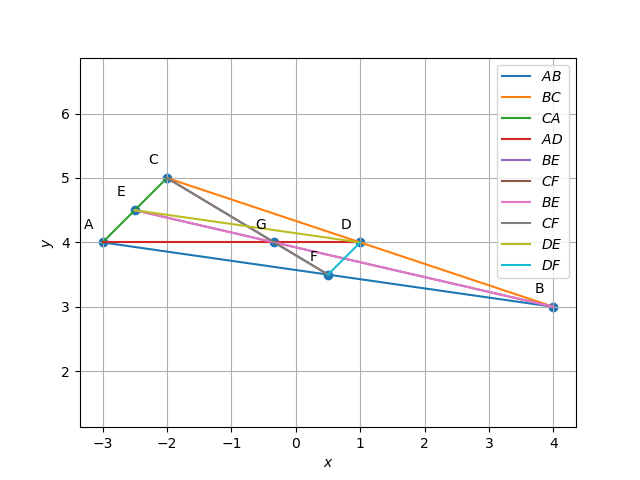
\includegraphics[width=\columnwidth] {./figs/fig18.png}
\caption{ Fig 2}
\label{fig2: midpoints}
\end{figure}

\begin{table}[h!]
 \begin{center}
  \caption{Table 3}
  \label{tab: table3}
\begin{tabular}{|l|c|r|}
     \hline
    Parameter & Values & Description\\
     \hline
     $\vec{n_1}$ & $\myvec{6\\-2\\}$ & Equation of\\
     ${c_1}$ & -26 & altitude $AP$\\
     $\vec{n_2}$ & $\myvec{1\\1\\}$ & Equation of\\
     ${c_2}$ & 7 & altitude $BQ$\\
     $\vec{n_3}$ & $\myvec{-7\\1\\}$ & Equation of\\
     ${c_3}$ & 19 & altitude $CR$\\
     \hline
     $\vec H$ & $\myvec{\frac{-3}{2}\\\frac{17}{2}\\}$ & orthocenter\\
     \hline
     {} & $(A-H)^T.(B-C)=0$ & Verified\\
     \hline
\end{tabular}
\end{center}
\end{table}
\begin{figure}[h!]
\centering

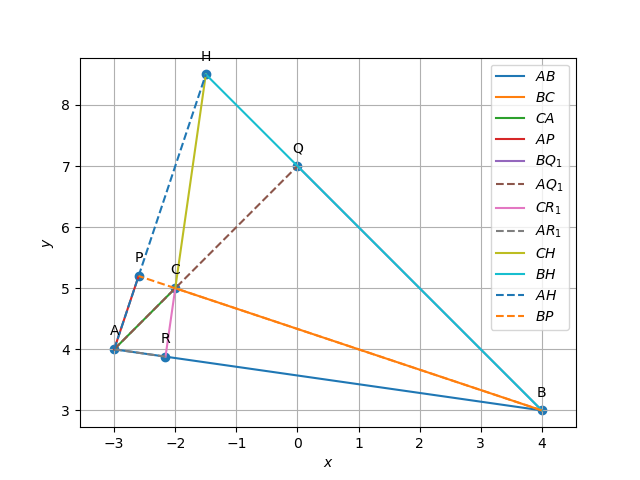
\includegraphics[width=\columnwidth] {./figs/fig19.png}
\caption{Figure 3}
\label{fig: $AP$}

\end{figure}

\begin{table}[h!]
 \begin{center}
  \caption{Table 4}
  \label{tab: table4}
\begin{tabular}{|l|c|r|}
     \hline
    Parameter & Values & Description\\
     \hline
     $\vec{n_1}$ & $\myvec{-6\\2\\}$ & Perpendicular bisector\\
     ${c_1}$ & 2 & of $BC$\\
     $\vec{n_2}$ & $\myvec{-1\\-1\\}$ & Perpendicular bisector\\
     ${c_2}$ & -2 & of $CA$\\
     $\vec{n_3}$ & $\myvec{7\\-1\\}$ & Perpendicular bisector\\
     ${c_3}$ & 0 & of $AB$\\
     \hline
     $\vec O$ & $\myvec{\frac{1}{4}\\\frac{7}{4}\\}$ & Circumcentre\\
     \hline
     {} & $(O-(B+C)/2).(B-C)=0$ & Verified\\
     \hline
     OA & 3.952 & $OA=OB=OC$\\
     OB & 3.952 & Hence verified\\
     OC & 3.952 & {}\\
     \hline
     $\angle BOC$ & $106.26\degree$ & $\angle BOC$=2 $\angle BAC$\\
     $\angle BAC$ & $53.13\degree$  & Verified\\
     \hline
\end{tabular}
\end{center}
\end{table}
\begin{figure}[h!]
\centering

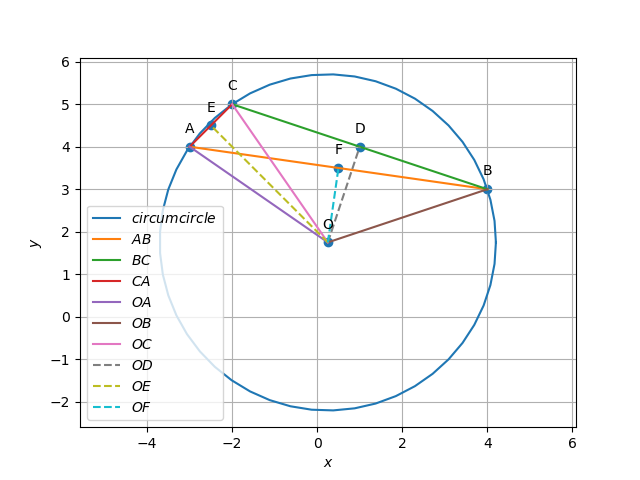
\includegraphics[width=\columnwidth] {./figs/fig20.png}
\caption{ Figure 4}
\label{fig: Perpendicular bisectors}

\end{figure}

\begin{table}[h!]
 \begin{center}
  \caption{Table 5}
  \label{tab: table5}
\begin{tabular}{|l|c|r|}
     \hline
    Parameter & Values & Description\\
     \hline
     $\vec{n_1}$ & $\myvec{0.57\\-1.7\\}$ & Angular bisector\\
     ${c_1}$ & -8.48 & of $\angle A$\\
     $\vec{n_2}$ & $\myvec{0.46\\1.94\\}$ & Angular bisector\\
     ${c_2}$ & 7.64 & of $\angle B$\\
     $\vec{n_3}$ & $\myvec{-1.02\\-0.24\\}$ & Angular bisector\\
     ${c_3}$ & 0.84 & of $\angle C$\\
     \hline
     $\vec I$ & \myvec{-1.85\\4.38\\} & Incenter\\
     \hline
     $\angle BAI$ &  $26.56\degree$ & $\angle BAI$=$\angle CAI$\\
     $\angle CAI$ & $26.56\degree$ & Verified\\
     \hline
     ${d_1}$ & $0.54$ & Distance between $I$ and $BC$\\
     ${d_2}$ & $0.54$ & Distance between $I$ and $CA$\\
     ${d_3}$ & $0.54$ & Distance between $I$ and $AB$\\
     \hline
     $D_3$ & $\myvec{-1.68\\4.89\\}$ & point of tangency by side $BC$\\
     $E_3$ & $\myvec{-2.24\\4.76\\}$ & point of tangency by side $CA$\\
     $F_3$ & $\myvec{-1.93\\3.85\\}$ & point of tangency by side $AB$\\
     \hline
     $AE_3$ & $1.08$ & $AE_3=AF_3=m$\\
     $AF_3$ & $1.08$ & {}\\
     $BD_3$ & $5.99$ & $BD_3=BF_3=n$\\
     $BF_3$ & $5.99$ & {}\\
     $CD_3$ & $0.33$ & $CD_3=CE_3=p$\\
     $CE_3$ & $0.33$ & {}\\
     \hline
     $m$ & $1.08$ & $m=(b+c-a)/2$\\
     $n$ & $5.99$ & $n=(c+a-b)/2$\\
     $p$ & $0.33$ & $p=(a+b-c)/2$\\
     \hline
\end{tabular}
\end{center}
\end{table}
\begin{figure}[h!]
\centering

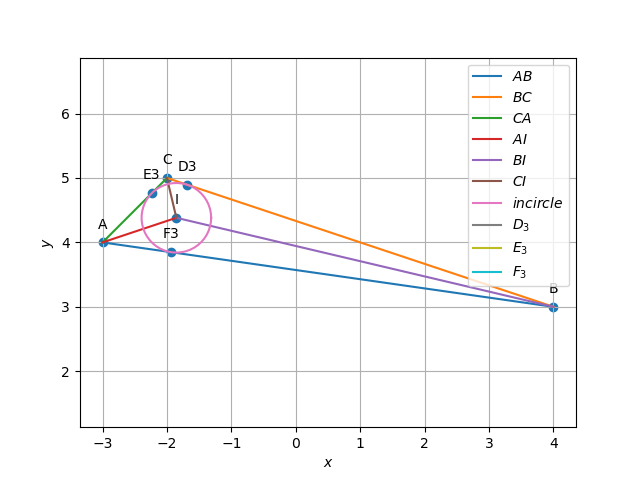
\includegraphics[width=\columnwidth]{./figs/fig21.png}
\caption{Figure 5}
\label{fig:Incenter}

\end{figure}
\end{document}

